% arara: pdflatex
% arara: pdflatex
% arara: pdflatex

% options:
% thesis=B bachelor's thesis
% thesis=M master's thesis
% czech thesis in Czech language
% slovak thesis in Slovak language
% english thesis in English language
% hidelinks remove colour boxes around hyperlinks

\documentclass[thesis=B,czech]{FITthesis}[2012/06/26]

\usepackage[utf8]{inputenc} % LaTeX source encoded as UTF-8

% My packages
\usepackage{hyperref}
\usepackage{xcolor}
\usepackage{listings}
\lstset{basicstyle=\ttfamily,
  showstringspaces=false,
  commentstyle=\color{red},
  keywordstyle=\color{blue}
}

\usepackage{graphicx} %graphics files inclusion
\graphicspath{ {./images/} }
% \usepackage{amsmath} %advanced maths
% \usepackage{amssymb} %additional math symbols

\usepackage{dirtree} %directory tree visualisation

% % list of acronyms
% \usepackage[acronym,nonumberlist,toc,numberedsection=autolabel]{glossaries}
% \iflanguage{czech}{\renewcommand*{\acronymname}{Seznam pou{\v z}it{\' y}ch zkratek}}{}
% \makeglossaries

\newcommand{\tg}{\mathop{\mathrm{tg}}} %cesky tangens
\newcommand{\cotg}{\mathop{\mathrm{cotg}}} %cesky cotangens

% % % % % % % % % % % % % % % % % % % % % % % % % % % % % % 
% ODTUD DAL VSE ZMENTE
% % % % % % % % % % % % % % % % % % % % % % % % % % % % % % 

\department{Katedra softewarového inženýrství}
\title{Věnná města českých královen - API~pro~předávání grafických modelů}
\authorGN{Martin} %(křestní) jméno (jména) autora
\authorFN{Čapek} %příjmení autora
\authorWithDegrees{Martin Čapek} %jméno autora včetně současných akademických titulů
\author{Martin Čapek} %jméno autora bez akademických titulů
\supervisor{Jiří Chludil}
\acknowledgements{Děkuji především své rodině za podporu, svému vedoucímu za časté konzultace a za směrování mě k práci.}
\abstractCS{Práce je věnována analýze funkčním a nefunkčním požadavkům editoru Virtuálního historického průvodce, který má zjednodušit práci odborníkům (zvláště historikům).



Hlavním přínosem této práce není vytvořit plně funkční REST API,
ač je implementován funkční prototyp, ale sestavit obsáhlý manuál, základní
kámen činnosti pro následující generace řešitelů projektu.}
\abstractEN{abstractEN}
\placeForDeclarationOfAuthenticity{V~Praze}
\declarationOfAuthenticityOption{4} %volba Prohlášení (číslo 1-6)
\keywordsCS{Node.js, RestAPI, PostgreSQL, virtuální realita, historické modely budov}
\keywordsEN{Nahraďte seznamem klíčových slov v angličtině oddělených čárkou.}
% \website{http://site.example/thesis} %volitelná URL práce, objeví se v tiráži - úplně odstraňte, nemáte-li URL práce

\begin{document}

% \newacronym{CVUT}{{\v C}VUT}{{\v C}esk{\' e} vysok{\' e} u{\v c}en{\' i} technick{\' e} v Praze}
% \newacronym{FIT}{FIT}{Fakulta informa{\v c}n{\' i}ch technologi{\' i}}

\begin{introduction}
	 Věnná města českých královen je rozsáhlý projekt, jehož cílem je vytvoření specializovaného historického průvodce věnnými městy a jejich městskou krajinou.
	 Momentálně se v tomto projektu vyvíjí editor virtuální reality, který má sloužit jako nástroj historikům a jiným odborníkům, ve kterém budou moci spolupracovat na vytváření modelů, zasazování modelů do krajiny a tím vytvářet historická věnná města. Účelem editoru bude sloužit i návštěvníkům si tato města prohlížet.

	 V mojí práci se věnuji analýze požadavků editoru virtuální reality, návrhem API pro editor, implementací jeho prototypu a otestováním prototypu.
	 
	 Uživatelé v editoru budou potřebovat API pro práci s velkým množstvím informací a garfických modelů, uložených v databázi. API bude také potřeba k řešení přístupových práv, protože některé informace jsou citlivé a s něterými modely mohou manipulovat jen určití lidé. 
	 Výsledek této bakalářské práce bude vzorem pro vývoj API v rámci projektu Věnná města českých královen.
\end{introduction}

\chapter{Cíl práce}

% ? jaky editoru virtuální reality?
    Cílem teoretické části práce je analyzovat funkční a nefunkční požadavky editoru virtuální reality. Při analýze se zaměřit na datové úložiště a způsob propagace modelů. Dále provést analýzu nástrojů pro návrh a dokumentaci API a z těchto nástrojů vybrat nejvhodnější a s jeho použitím navrhnout prototyp API, které umožní komunikaci mezi datovým úložištěm a editorem virtuální reality.
    Dalším cílem práce je popsat vývojové prostředí, které využiji v implementaci. V popisu budou použité technologie, příprava vývojářského prostředí a doporučený způsob verzování zdrojových kódů.
    
    Cílem praktické části práce je implementace a otestování prototypu REST API za použití technologie Node.js a využítím technologie continuous integration.


\chapter{Analýza}
    \section{Požadavky editoru virtuální reality}
        \subsection{Funkční}
        \label{sec:analFP}
% todo upravit
            Následující sekce popisuje funkční požadavky editoru virtuální reality. Tedy požadavky, které se vztahují k funkcionalitě na cílovou aplikaci. Tyto požadavky jsem vytvořil s pomocí Patrika Křepinského.
            \begin{itemize}
                \item Přihlášení
                
                V aplikaci musí být možnost přihlášení. Pokud se nepřihlásíte, můžete pokračovat jako host, který nemá žádná práva na grafické modely, tedy si je můžete pouze prohlížet.
                \item Odhlášení
                
                Stejně jako přihlášení je nutná možnost odhlášení. Dále je potřeba mít možnost zůstat trvale přihlášen na tomto počítači, jinak funguje automatické odhlášení po ukončení aplikace.
               \item Práva k modelu
               
                Model má svého autora a dále skupinu uživatelů, kteří mají některá z následujících práv:
                \begin{itemize}
                    \item pouze čtení a zobrazení
                    \item čtení a zobrazení s možností psaní komentářů?
                    \item měnění poznámek a metadat (popis)
                    \item editace modelu
                    \item kopírování modelu pro svoje potřeby (povolení vytvořit na základě modelu jiný model)
                    \item plná práva
                \end{itemize}
                Tuto skupinu uživatelů může autor libovolně editovat. Pokud uživatel není ve skupině znamená to, že nemá žádná práva k tomuto modelu.
               \item Práva k projektu
               
                Projekt je skupina modelů zasazená do lokace. Takovým projektem může být historický model města. Projekt má skupinu uživatelů, kteří mají některá z následujících práv:
                \begin{itemize}
                    \item Změna lokace modelu
                    \item Nahrávání
                    \item Mazání
                    \item Udělovat práva
                    \item Seskupení
                \end{itemize}
                Uživatel bude moct zařadit model do skupiny. Tato funkce poslouží k lepší organizaci pracovního prostředí.
                \item Žádosti o práva
                
                Dále mohou uživatelé žádat o určitá práva k modelu nebo skupině modelů a k projektu. Tuto žádost mohou autoři potvrdit.
                \item Zobrazení miniatur po přihlášení
                
                Je třeba, aby po přihlášení měl uživatel přístup ke svým modelům. To umožní naše aplikace v podobě miniatur grafických modelů, které se po přihlášení načtou.
                \item Třídění miniatur
                
                Tyto miniatury si bude moct uživatel třídit podle stavu modelů, přístupových práv, skupin uživatelů, atd.
                \item Zobrazení modelů projektu v určitém čase a počasí
                
                Uživatel si bude moct zobrazit celý projekt v nějakém čase a procházet si ho. Bude si moct nastavovat počasí a denní dobu. Bude si ho moci procházet i napříč historií.
                \item Ulož všechny změny v projektu
                
                Uživatel potvrdí a uloží provedené změny na server. Po tomto uložení uvidí změny všichni kdo mají k modelu přístup.
                U modelu máme dva základní typy změn:
                \begin{itemize}
                    \item transformace (rotace, translace, scale)
                    \item informace o modelu (poznámka, autorství)
                \end{itemize}
                \item Vytvoř kopii modelu
                
                Uživatel bude moct vytvořit model na základě nějakého jiného modelu (pokud k tomu bude mít právo), aby nemusel začínat od začátku.
                \item Přidání modelu do projektu
                
                Pokud bude moct uživatel editovat nějaký projekt, může přidávat i nové modely.
               \item Vytvoř kopii projektu
               
                Uživatel vytvoří kopii projektu, pokud k tomu má právo, aby mohl provádět nějaké experimentální úpravy.
               \item Smaž model
               
                Uživatel smaže model pro který už nemá žádné využití. Po kliknutí na smazání modelu se aplikace ještě zeptá, jestli si je opravdu jist, protože grafický model může představovat desítky hodin práce a může se stát, že uživatel klikne na tlačítko smazat omylem.
                \item Vytvoř nový model
                
                Uživateli se zobrazí prázdná pracovní plocha, kde bude moct vymodelovat nový model.
                \item Vytvoř nový projekt
                
                Uživatel vytvoří prázdnou pracovní plochu, kam bude moct zasazovat modely.
                Nahrání modelu z lokálního zařízení
                Uživatel nahraje model z disku a může ho uložit na server.
            \end{itemize}
        \subsection{Nefunkční}
% todo upravit
            Tato sekce se zabývá nefunkčními požadavky na REST API. Tedy požadavky, které se zaměřují na nároky cílové aplikace na software a to například z hlediska bezpečnosti, spolehlivosti, či výkonu.
            \begin{itemize}
                \item Rychlost odezvy

                    Uživatel nesmí na obdržení nebo aktualizování grafického modelu čekat. Je třeba, aby server reagoval rychle.
                \item Datová nenáročnost při komunikaci

                    Je třeba minimalizovat množství dat posílané přes API, abychom docílili rychlosti a zbytečně nepřetěžovali spojení s koncovým uživatelem.
                \item Bezpečnost
                    
                    Určité koncové body vyžadují oprávnění, jelikož jejich zavoláním se předávají nebo přepisují citlivá data. To se vyřeší tím, že při přihlášení dostane uživatel token, kterým se bude autorizovat u volání citlivých koncových bodů.
                \item Rozšiřitelnost

                    API musí umožňovat případné rozšíření o další funkcionality. Také musí být řádně zdokumentováno, aby umožnilo hladší průběh rozšiřování.
                \item Použité technologie

                    Bylo zadáno, že se bude vyvýjet v technologii Node.js za využití modulu Express.
            \end{itemize}
    \section{Použité technologie}
        \subsection{Node.js}
            Node.js je open-source multiplatformní JavaScriptové prostředí postaveno na Chrome V8 JavaScript enginu. Primární účel Node.js je tvorba serverové části webových aplikací, které vychází z paradigmatu "JavaScript everywhere".
            
            Node.js využívá událostmi řízenou architekturu a neblokující I/O operace. Tento návrh optimalizuje výkon a škálovatelnost programů s častými požadavky na I/O operace.
            
            Jádro celého Node.js tvoří smyčka událostí, která běží na jednom vlákně. Ta podporuje desetitisíce souběžných připojení bez nutnosti neustálého přepínání kontextu díky neblokujícímu I/O. Nedochází zde k žádnému zamykání, tudíž nemusíme mít obavy z deadlocku systému.
        \subsection{npm}
            Node.js využívá správce balíčků npm, jehož pomocí můžeme obecně instalovat i spravovat závislosti a spouštět skripty. Npm se chlubí tím, že je největším balíčkovacím správcem a aktuálně obsahuje skoro 800 000 balíčků. - zdroj http://www.modulecounts.com.
        \subsection{Express}
            Express je framework pro Node.js, který nám umožnuje jednoduše napsat webovou aplikaci, či API. Těší se velké popularitě, momentálně na 4. místě npm rank\footnote{https://gist.github.com/anvaka/8e8fa57c7ee1350e3491}.
        \subsection{JWT} \label{jwt}
            JWT (JSON Web Token) je standart, který zajišťuje bezpečný přesun informací zapsaných v JSON.
            \begin{figure}[ht!]
                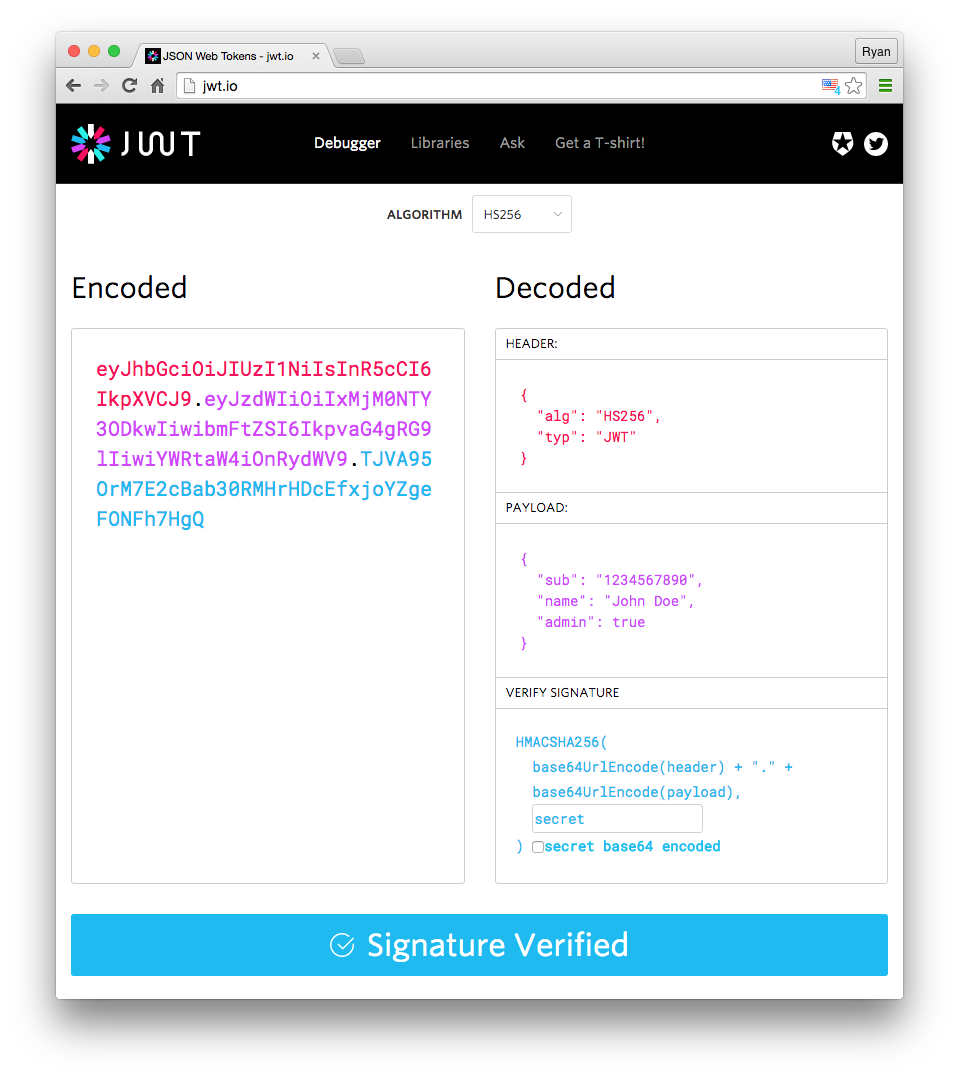
\includegraphics[scale=0.4]{legacy-app-auth-5}
                \caption{JWT}
            \end{figure}
            
            JWT se skládá ze 3 částí:
            \begin{itemize}
                \item Header
                    
                    obsahuje typ tokenu a šifrovací algoritmus.
                \item Payload
                    
                    obsahuje naše informace a může obsahovat ještě dodatečné informace jako expirace tokenu, vydavatel atd. % vydavatel = issuer
                \item Signature
                    
                    obsahuje zakódované předešlé části a secret -- náš tajný klíč.
            \end{itemize}
             V naší aplikaci využijeme tuto technologii pro ověřování totožnosti uživatelů. Naše aplikace vytvoří JWT po přihlášení a uživatel se jím bude nadále identifikovat
            \begin{figure}[ht!]
                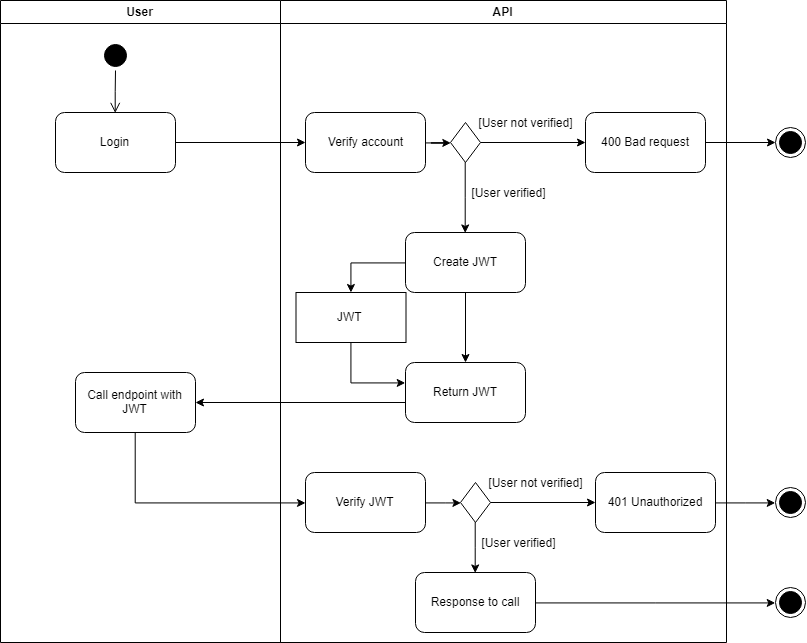
\includegraphics[scale=0.45]{Process_of_authentication}
                \caption{Proces autorizace}
            \end{figure}
        \subsection{Implementační jazyk}
            Pro vývoj byl vybrán jazyk TypeScript, který je kompilovatelný do JavaScriptu. Tento jazyk je vyvýjen firmou Microsoft a jeho hlavní myšlenkou je být nadstavbou JavaScriptu, která přidává statické typování a další funkcionalitu.
        \subsubsection{TSLint}
            TSLint je nástroj pro statickou analýzu kódu TypeScriptu.
        \subsection{PostgreSQL}
            Pro datovou vrstvu byla vybrána databáze PostgreSQL.
            
            PostgreSQL je objektově-relační databázový systém pod MIT licencí. Je pověstný svou spolehlivostí a vysokou bezpečností. Na PostgreSQL wiki\footnote{\url{https://wiki.postgresql.org/wiki/Community_Guide_to_PostgreSQL_GUI_Tools}} lze nalézt rozsáhlý seznam dostupného open-source software, sloužícího k administraci a monitoringu PostgreSQL databází. Nejrozšířenější a velmi přehledný je pgAdmin.
        \subsection{TypeORM}
            \url{https://typeorm.io}
        
        
            Jak již název napovídá jedná se o objektově relační mapování, což nám umožní jednodušeji pracovat s databází. TypeORM podporuje PostgreSQL a má npm balíček, který budeme moci využít při implementaci v Node.js.
            
        \subsection{Dotenv}
            \url{https://github.com/motdotla/dotenv}
            
            Tato knihovna umožňuje pracovat s proměnými prostředí
    \section{Nástroje pro návrh REST API}
        \subsection{Swagger}
            Swagger je sada nástrojů postavená na OpenAPI Specifikaci.
            \newline Nástroje:
            \begin{itemize}
                \item Swagger editor - webový editor umožňující psát OpenAPI Specifikace
                \item Swagger UI - vizualizuje API dokumentaci, kterou generuje z OpenAPI Specifikace
                \item Swagger Codegen - vygeneruje kód na základě OpenAPI Specifikace
            \end{itemize}
            OpenAPI Specifikace, dřívěji Swagger Specifikace, je sada pravidel, které sémanticky popisují API. Pravidla mohou být zapsaná nebo vygenerována do souboru formátu YAML, nebo JSON. YAML je více čitelný pro lidi, kteří nejsou zvyklí na závorky. Programátorům může více vyhovovat JSON. OpenAPI~Specifikace se skládá z metadat, koncových bodů a schématu.
        \subsection{Apicurio Studio}
            Apicurio Studio je open-source editor pro OpenAPI specifikaci. Musíte se přihlásit a vaše návrhy REST API se ukládají do vašeho repozitáře na GitHubu, GitLabu nebp Bitbucketu, což se hodí v případě, když na návrhu pracujete spolčně v týmu. V editoru můžete přepínat mezi interaktivní vizualizací návrhu a jeho JSON/YAML definicí.
        \subsection{RAML}
            RAML je akronym RESTful API Modeling Language a je to typ souboru podobný YAML. Existují různé nástroje používající RAML, vypíši některé z těch nástrojů:
            \href{http://apiworkbench.com}{API Workbench} je IDE pro RAML, které je v beta verzi a funguje jako balíček pro Atom, což je teztový editor.
            \href{https://github.com/raml2html/raml2html}{Raml2html} dokáže z RAML vytvořit  HTML dokumentaci.
            \href{https://github.com/mulesoft/osprey}{Osprey} dokáže z RAML vygenerovat API pro Node.js.
        \subsection{Restlet}
            Restlet Studio je webová aplikace, která umožňuje uživateli interaktivně upravovat REST API. Doáže definované API exportovat do OpenAPI specifikace nebo RAML. Dokáže vytvořit  Server Skeleton pro Node.js.
        \subsection{Apiary}
            Api editor podporuje API Blueprint i OpenAPI Specifikaci.
            
            API Blueprint je podobně jako OpenAPI Specifikace sada pravidel popisující API. API Blueprint specifikace je zapsaná v Markdown dokumentu, který je rozdělen do sekcí. Tyto sekce nejsou povinné.
            
            Výpis základních 5 sekcí, u každé je číslo, které vyjadřuje kolikrát se sekce může v dokumentu objevit.
            \begin{itemize} % je angličtina v pohode?
                \item 0-1 Metadata
                \item 0-1 API Name \& overview
                \item 0+ Resource
                \item 0+ Resource Group
                \item 0+ Data Structures
            \end{itemize}
            
            Apiary disponuje interaktivní dokumentací, webový editor má možnost přepnutí do tmavého režimu. Dále zajišťuje propojení s GitHub nebo GitLab repozitářem.

    \section{Výběr nástroje pro návrh a dokumentaci API}
        V této sekci navážu na předešlou analýzu nástrojů pro návrh REST API a vyberu zde nejvhodnější nástroj. Nejvíce mě nadchnul Swagger a Apiary, popíši zde porovnání těchto nástrojů.
        

        Oba nástroje jsem vyzkoušel, Swagger jsem zkoušel ve SwaggerHubu, což je webová aplikace, která přináší všechny základní vlastonsi Swaggeru. Oba nástroje umožnují požadovanou dokumentaci a návrh API a k tomu i generování kódu.
        
        Co jse mi na Swaggeru líbilo a v Apiary chybělo je, že vizualizovaná dokumentace měla označené zabezpečené koncové body, dokumentace se dá exportovat do html, editor obsahuje navigátora, který umožnuje přeskakovat do různých sekcí dokumentu a náhled dokumentace také odkazuje na části dokumentu, takže se k nim jde jednoduše "prokliknout". Zpřehlednění orientace v dokumnetu, jež SwaggerHub nabízí, je velice vhodné, protože dokumentace API čítá bežně stovky až tisíce řádků.
        
        Apiary nemá žádný export, existuje ale Apiary CLI, které umožnuje zobrazit dokumentaci v internetovém prohlížeči.
                
        \subsection{OpenAPI Specifikace vs API Blueprint}
            Markatní rozdíl mezi nimi je, že Swagger je težce provázán s OpenAPI Specifikací, kdežto Apiary, přestože podporuje OpenAPI Specifikaci, je založeno na API Blueprintu.

            Při porovnání repozitářů \href{https://github.com/apiaryio/api-blueprint/graphs/contributors}{API Blueprint} a \href{https://github.com/OAI/OpenAPI-Specification/graphs/contributors}{OAS} můžeme vidět, že OpenAPI Specifikace je více živější, co se týče commitů i řešených problémů, navíc má zhruba dvakrát více hvězdiček a forků.
            
            OAS je založený na YAML (nebo JSON) formátu a API Blueprint má vlastní formát APIB, který má syntaxi podobnou Markdownu a využívá MSON\footnote{\url{https://github.com/apiaryio/mson}}. Rozdíl v těchto formátech je spíše otázka osobního vkusu, jelikož se líší především syntaxí.
        \subsection{Závěr}
            Oba nástroje jsou srovnatelné, ale Swagger nabízí více možností pracování s dokumnetací a hlavně proto jsem se rozhodl ho nominovat jako vítěze tohoto pomyslného souboje.

\chapter{Návrh}
    V této kapitole provedu návrh REST API na základě \hyperref[sec:analFP]{analýzy funkčních požadavků}. Funkční požadavky Odhlášení a Třídění miniatur nebudeme řwšit v tomto návrhu, protože se o ně postará TODO Editor. Odhlášení se provede v aplikaci odstraněním \hyperref[sec:jwt]{JWT}. Třídění miniatur následuje po Zobrazení miniatur po přihlášení, miniatury tedy budou uloženy v aplikaci a o jejich třídení se postará aplikace. Ostatní funkčí požadavky jsem uvedl v \hyperref[sec:tabulkaPokryti]{tabulce pokrytí funkčních požadavků}, kde ke každému požadavku je uveden koncový bod API.
    
    Na základě \hyperref[sec:tabulkaPokryti]{této tabulky} jsem vytvořil návrh ve Swaggeru viz příloha.
    
    \begin{table}\centering
    	\caption{Pokrytí funkčních požadavků} \label{tabulkaPokryti}
    	\begin{tabular}{| p{6cm} | p{5cm} |}\hline
    		Funkční požadavek		& API endpoint	\tabularnewline \hline \hline
            Přihlášení & GET /login
        	\tabularnewline \hline
            Smaž model &	DELETE /model
        	\tabularnewline \hline
            Vytvoř nový model &	PUT /model
        	\tabularnewline \hline
            Editovat práva k modelu &	POST /model/\{modelId\}
        	\tabularnewline \hline
            Editovat práva k projektu &	POST /project/\{projectlId\}
        	\tabularnewline \hline
            Seskupení & POST /group/\{groupId\}
        	\tabularnewline \hline
            Žádosti o práva & GET /rights/model/\{modelId\}
        	\tabularnewline \hline
            Zobrazení miniatur po přihlášení & GET /miniatures
        	\tabularnewline \hline
            Zobrazení modelů projektu v určitém čase a počasí &
            \parbox[t]{5cm}{GET /model/\{modelId\}/time/\\\{time\}/weather/\{weather\}}
        	\tabularnewline \hline
            Ulož všechny změny v projektu &	POST /project/\{projectlId\}
        	\tabularnewline \hline
            Vytvoř kopii modelu	& PUT /model
        	\tabularnewline \hline
            Přidání modelu do projektu & POST /project/\{projectlId\}
        	\tabularnewline \hline
            Vytvoř nový projekt & PUT /project
        	\tabularnewline \hline
            Vytvoř kopii projektu &	PUT /project
        	\tabularnewline \hline
            Nahrání modelu z lokálního zařízení & PUT /project
        	\tabularnewline \hline
        \end{tabular}
    \end{table}

\chapter{Vývojářské prostředí pro OS~Linux}
    \section{Příprava vývojářského prostředí}
        \subsection{Node.js}
            \begin{lstlisting}[language=bash,caption={Instalace Node.js a npm}]
            sudo apt install nodejs --Yes
            sudo apt install npm --Yes
            \end{lstlisting}
            V implementaci je použita verze nodejs 8.10.0 a npm 3.5.2. Vaši verzi si můžete zkontrolovat pomocí následujích příkazů.
            \begin{lstlisting}[language=bash,caption={Zkontrolování verze Node.js a npm}]
            nodejs -v
            npm -v
            \end{lstlisting}

            Příkaz npm init -y nám vygeneruje jednoduchý package.json.
            Dále budeme instalovat balíčky. Po příkazu \textit{npm i název balíčku} (viz command npm help i) se nám balíček stáhne i s knihovnami, na kterých závisí, do složky node\_modules a taky se nám zapíše do package.json ve fomátu "název": "verze". U příkazu \textit{npm i} můžeme přidat \textit{--save-dev}, tímto označíme balíček, že není potřeba pro běh samotné aplikace, takto označíme balíčky potřebné pro vývoj a testování např. tslint, jest.


            npm i express nám nainstaluje Express.
            
            npm i --save-dev typescript nainstaluje typescript.
            
            npm i --save-dev tslint nainstaluje tslint
            
            Vytvoříme si tsconfig.json viz \url{https://www.typescriptlang.org/docs/handbook/tsconfig-json.html}.

            npm i --save-dev @types/node @types/express

        \subsection{PostgreSQL}
            TBD
    \section{Verzování}
        Tady popíšu doporučený způsob verzování zdrojových kódů.

\chapter{Implementace}

\chapter{Testování}

\begin{conclusion}
    % Zaobirat se cilem prakticke casti, dale lze napsat: aplikace by mohla....
\end{conclusion}

\bibliographystyle{csn690}
\bibliography{mybibliographyfile}

\appendix

\chapter{Seznam použitých zkratek}
% \printglossaries
\begin{description}
	\item[API] Application Programming Interface
	\item[I/O] Input/Output
	\item[npm] Node.js package manager
	\item[IDE] Integrated Development Environment
	\item[JSON] JavaScript Object Notation
	\item[OAS] OpenAPI Specification
	\item[CI] Continuous Integration
\end{description}


% % % % % % % % % % % % % % % % % % % % % % % % % % % % 
% % Tuto kapitolu z výsledné práce ODSTRAŇTE.
% % % % % % % % % % % % % % % % % % % % % % % % % % % % 
% 
% \chapter{Návod k~použití této šablony}
% 
% Tento dokument slouží jako základ pro napsání závěrečné práce na Fakultě informačních technologií ČVUT v~Praze.
% 
% \section{Výběr základu}
% 
% Vyberte si šablonu podle druhu práce (bakalářská, diplomová), jazyka (čeština, angličtina) a kódování (ASCII, \mbox{UTF-8}, \mbox{ISO-8859-2} neboli latin2 a nebo \mbox{Windows-1250}). 
% 
% V~české variantě naleznete šablony v~souborech pojmenovaných ve formátu práce\_kódování.tex. Typ může být:
% \begin{description}
% 	\item[BP] bakalářská práce,
% 	\item[DP] diplomová (magisterská) práce.
% \end{description}
% Kódování, ve kterém chcete psát, může být:
% \begin{description}
% 	\item[UTF-8] kódování Unicode,
% 	\item[ISO-8859-2] latin2,
% 	\item[Windows-1250] znaková sada 1250 Windows.
% \end{description}
% V~případě nejistoty ohledně kódování doporučujeme následující postup:
% \begin{enumerate}
% 	\item Otevřete šablony pro kódování UTF-8 v~editoru prostého textu, který chcete pro psaní práce použít -- pokud můžete texty s~diakritikou normálně přečíst, použijte tuto šablonu.
% 	\item V~opačném případě postupujte dále podle toho, jaký operační systém používáte:
% 	\begin{itemize}
% 		\item v~případě Windows použijte šablonu pro kódování \mbox{Windows-1250},
% 		\item jinak zkuste použít šablonu pro kódování \mbox{ISO-8859-2}.
% 	\end{itemize}
% \end{enumerate}
% 
% 
% V~anglické variantě jsou šablony pojmenované podle typu práce, možnosti jsou:
% \begin{description}
% 	\item[bachelors] bakalářská práce,
% 	\item[masters] diplomová (magisterská) práce.
% \end{description}
% 
% \section{Použití šablony}
% 
% Šablona je určena pro zpracování systémem \LaTeXe{}. Text je možné psát v~textovém editoru jako prostý text, lze však také využít specializovaný editor pro \LaTeX{}, např. Kile.
% 
% Pro získání tisknutelného výstupu z~takto vytvořeného souboru použijte příkaz \verb|pdflatex|, kterému předáte cestu k~souboru jako parametr. Vhodný editor pro \LaTeX{} toto udělá za Vás. \verb|pdfcslatex| ani \verb|cslatex| \emph{nebudou} s~těmito šablonami fungovat.
% 
% Více informací o~použití systému \LaTeX{} najdete např. v~\cite{wikilatex}.
% 
% \subsection{Typografie}
% 
% Při psaní dodržujte typografické konvence zvoleného jazyka. České \uv{uvozovky} zapisujte použitím příkazu \verb|\uv|, kterému v~parametru předáte text, jenž má být v~uvozovkách. Anglické otevírací uvozovky se v~\LaTeX{}u zadávají jako dva zpětné apostrofy, uzavírací uvozovky jako dva apostrofy. Často chybně uváděný symbol "{} (palce) nemá s~uvozovkami nic společného.
% 
% Dále je třeba zabránit zalomení řádky mezi některými slovy, v~češtině např. za jednopísmennými předložkami a spojkami (vyjma \uv{a}). To docílíte vložením pružné nezalomitelné mezery -- znakem \texttt{\textasciitilde}. V~tomto případě to není třeba dělat ručně, lze použít program \verb|vlna|.
% 
% Více o~typografii viz \cite{kobltypo}.
% 
% \subsection{Obrázky}
% 
% Pro umožnění vkládání obrázků je vhodné použít balíček \verb|graphicx|, samotné vložení se provede příkazem \verb|\includegraphics|. Takto je možné vkládat obrázky ve formátu PDF, PNG a JPEG jestliže používáte pdf\LaTeX{} nebo ve formátu EPS jestliže používáte \LaTeX{}. Doporučujeme preferovat vektorové obrázky před rastrovými (vyjma fotografií).
% 
% \subsubsection{Získání vhodného formátu}
% 
% Pro získání vektorových formátů PDF nebo EPS z~jiných lze použít některý z~vektorových grafických editorů. Pro převod rastrového obrázku na vektorový lze použít rasterizaci, kterou mnohé editory zvládají (např. Inkscape). Pro konverze lze použít též nástroje pro dávkové zpracování běžně dodávané s~\LaTeX{}em, např. \verb|epstopdf|.
% 
% \subsubsection{Plovoucí prostředí}
% 
% Příkazem \verb|\includegraphics| lze obrázky vkládat přímo, doporučujeme však použít plovoucí prostředí, konkrétně \verb|figure|. Například obrázek \ref{fig:float} byl vložen tímto způsobem. Vůbec přitom nevadí, když je obrázek umístěn jinde, než bylo původně zamýšleno -- je tomu tak hlavně kvůli dodržení typografických konvencí. Namísto vynucování konkrétní pozice obrázku doporučujeme používat odkazování z~textu (dvojice příkazů \verb|\label| a \verb|\ref|).
% 
% \begin{figure}\centering
% 	
\includegraphics[width=0.5\textwidth, angle=30]{cvut-logo-bw}
% 	\caption[Příklad obrázku]{Ukázkový obrázek v~plovoucím prostředí}\label{fig:float}
% \end{figure}
% 
% \subsubsection{Verze obrázků}
% 
% % Gnuplot BW i barevně
% Může se hodit mít více verzí stejného obrázku, např. pro barevný či černobílý tisk a nebo pro prezentaci. S~pomocí některých nástrojů na generování grafiky je to snadné.
% 
% Máte-li například graf vytvořený v programu Gnuplot, můžete jeho černobílou variantu (viz obr. \ref{fig:gnuplot-bw}) vytvořit parametrem \verb|monochrome dashed| příkazu \verb|set term|. Barevnou variantu (viz obr. \ref{fig:gnuplot-col}) vhodnou na prezentace lze vytvořit parametrem \verb|colour solid|.
% 
% \begin{figure}\centering
% 	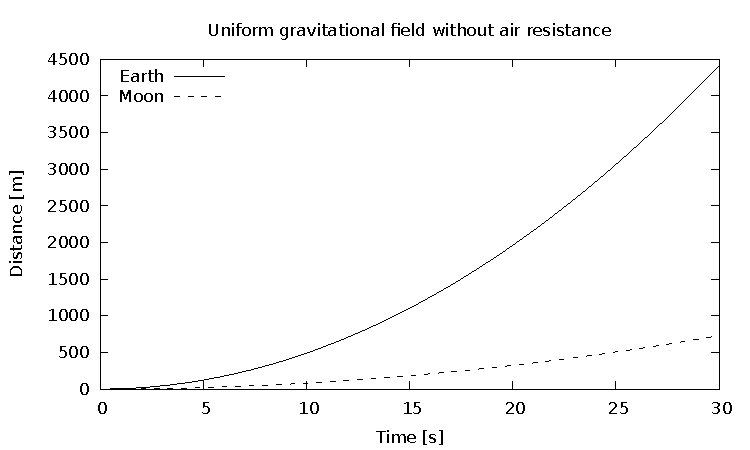
\includegraphics{gnuplot-bw}
% 	\caption{Černobílá varianta obrázku generovaného programem Gnuplot}\label{fig:gnuplot-bw}
% \end{figure}
% 
% \begin{figure}\centering
% 	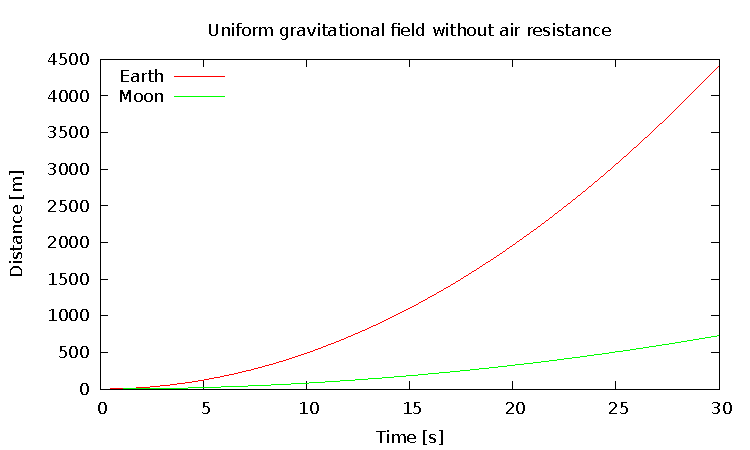
\includegraphics{gnuplot-col}
% 	\caption{Barevná varianta obrázku generovaného programem Gnuplot}\label{fig:gnuplot-col}
% \end{figure}
% 
% 
% \subsection{Tabulky}
% 
% Tabulky lze zadávat různě, např. v~prostředí \verb|tabular|, avšak pro jejich vkládání platí to samé, co pro obrázky -- použijte plovoucí prostředí, v~tomto případě \verb|table|. Například tabulka \ref{tab:matematika} byla vložena tímto způsobem.
% 
% \begin{table}\centering
% 	\caption[Příklad tabulky]{Zadávání matematiky}\label{tab:matematika}
% 	\begin{tabular}{|l|l|c|c|}\hline
% 		Typ		& Prostředí		& \LaTeX{}ovská zkratka	& \TeX{}ovská zkratka	\tabularnewline \hline \hline
% 		Text		& \verb|math|		& \verb|\(...\)|	& \verb|$...$|		\tabularnewline \hline
% 		Displayed	& \verb|displaymath|	& \verb|\[...\]|	& \verb|$$...$$|	\tabularnewline \hline
% 	\end{tabular}
% \end{table}
% 
% % % % % % % % % % % % % % % % % % % % % % % % % % % % 

\chapter{Obsah přiloženého CD}

%upravte podle skutecnosti

\begin{figure}
	\dirtree{%
		.1 readme.txt\DTcomment{stručný popis obsahu CD}.
		.1 exe\DTcomment{adresář se spustitelnou formou implementace}.
		.1 src.
		.2 impl\DTcomment{zdrojové kódy implementace}.
		.2 thesis\DTcomment{zdrojová forma práce ve formátu \LaTeX{}}.
		.1 text\DTcomment{text práce}.
		.2 thesis.pdf\DTcomment{text práce ve formátu PDF}.
		.2 thesis.ps\DTcomment{text práce ve formátu PS}.
	}
\end{figure}

\end{document}
